\documentclass[12pt]{article}
\usepackage{amsmath}
\usepackage{graphicx}
\usepackage{hyperref}
\usepackage[latin1]{inputenc}

\title{Pairwise shortest distance of honeycomb}
\author{Zhihao Wang}

\begin{document}
\maketitle

\section{Problem}

\begin{center}
  \makebox[\textwidth]{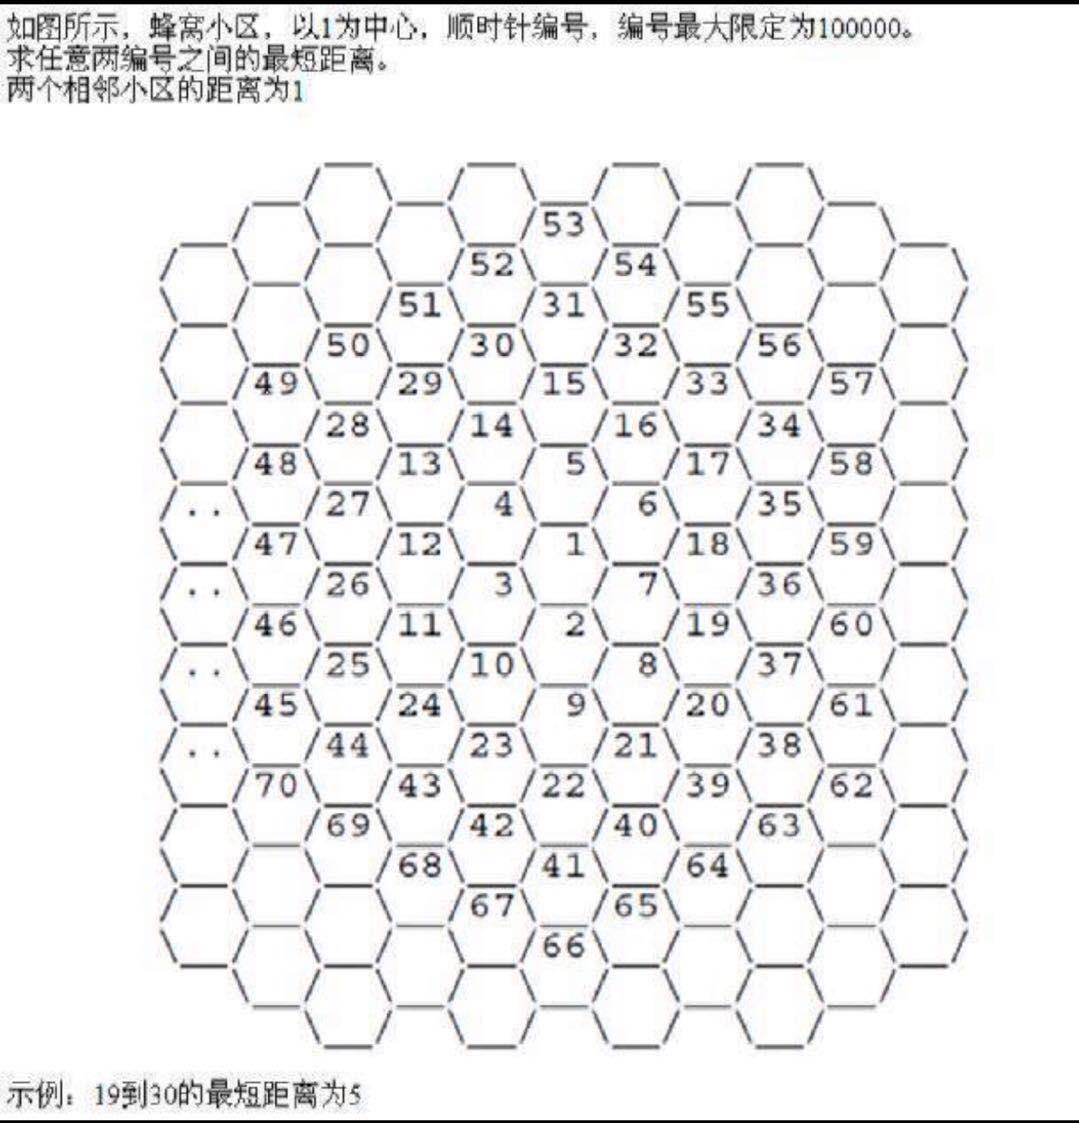
\includegraphics[width=0.5\paperwidth]{original-problem.jpg}}
\end{center}

\section{Solution}
We can add two axies and skew the honeycomb to get a cartesian coordinate system.

\begin{center}
  \makebox[\textwidth]{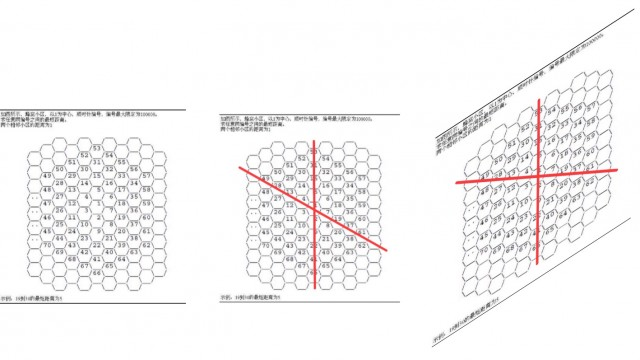
\includegraphics[width=0.5\paperwidth]{skew.jpg}}
\end{center}

Then we can calculate the coordinates as the following. Starting from some special coordinates, we can simulate the other coordinates case by case.

\begin{center}
  \makebox[\textwidth]{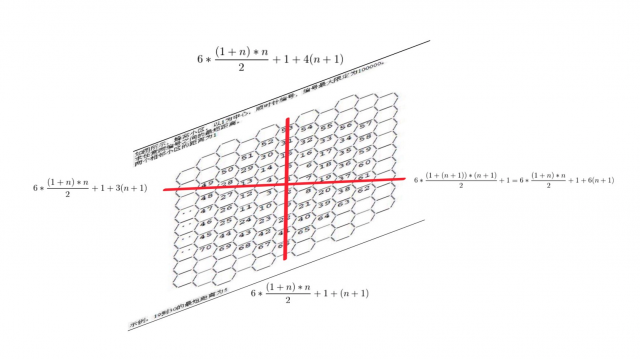
\includegraphics[width=0.5\paperwidth]{special-case-coordinates.png}}
\end{center}

Find the mininum $n$ and $ 0 \le p \le 5$ and $0 \le q \le n$

  \[
   Number = 6*\frac{(1+n)*n}{2} + 2 + p(n + 1) + q
  \]
 
Then the coordinate will be 
  \[
    Coordinate = \left\{\begin{array}{@{}lr@{}}
        (n - q, -1 - q), & \text{for }p = 0\\
        (-1 - q , -1 - n), & \text{for }p = 1\\
        (-1 - n, -n + q), & \text{for }p = 2\\
        (-n + q, 1 + q), & \text{for }p = 3\\
        (1 + q, 1 + n), & \text{for }p = 4\\
        (1 + n, n - q), & \text{for }p = 5
        \end{array}
  \]

We will have three operators in the new coordinate system, go horizontal, go veritical, and go 45 degree diagonal line, and there are two solutions.

\begin{center}
  \makebox[\textwidth]{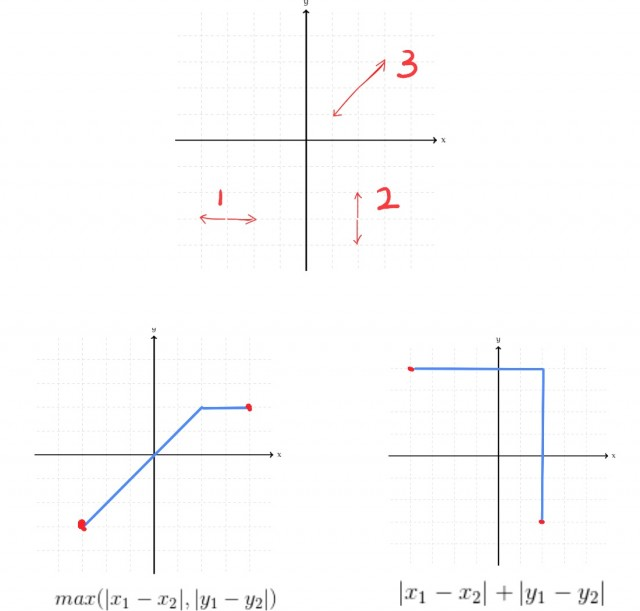
\includegraphics[width=0.5\paperwidth]{solution.jpg}}
\end{center}

Thanks to xinyu, he told me the answer are actually a mixture of Chebyshev distance and Manhattan distance, which is quite interesting especially when I found out Chebyshev distance is L_{\infty} distance and Manhattan distance is L_{1} distance.

\end{document}
